\subsection*{Hàm số}
\textbf{Bài 1.1:} Tìm miền xác định của các hàm số sau
\begin{enumerate}[label=(\alph*)]
\item \(\frac{x-2}{2x-1}\)
\item \(\frac{\ln(1+x)}{x-1}\)
\item \(\sqrt{1-2x}+3\arcsin\left(\frac{3x-1}{2}\right)\) \quad (\(\sin{x}=y\leftrightarrow x=\arcsin y\))
\item \(\frac{1}{x e^x}\)
\item \(\ln{(3x+1)}+2\ln{(x+1)}\)
\end{enumerate}

\vspace{5pt}
\textbf{Bài 1.2:} Tìm tập hợp giá trị của các hàm số sau
\begin{enumerate}[label=(\alph*)]
\item \(x^2 -6x+5\)
\item \(2+3\sin x\)
\item \(|x| + x + 1 = y + |y|\)
\item \(4^{-x^2}\)
\end{enumerate}
\vspace{5pt}

\textbf{Bài 1.3:} Chứng minh
\begin{enumerate}[label=(\alph*)]
\item $\sin(\alpha+\beta)=\sin\alpha\cos\beta + \sin\beta\cos\alpha.$
\item $\cos(\alpha+\beta)=\cos\alpha\cos\beta - \sin\alpha\sin\beta.$
\end{enumerate}

\emph{Gợi ý:} \href{https://vi.wikipedia.org/wiki/%C4%90%E1%BB%8Bnh_l%C3%BD_Ptoleme}{Định lý Ptoleme}

\subsection*{Vẽ đồ thị của hàm}
\emph{Chú ý}: Ta có thể vẽ đồ thị của hàm có dạng $y=Af(k(x-a))+b$ theo đồ thị của hàm $f(x)$
\begin{itemize}
    \item $y=f(x-a)$: đồ thị ban đầu được tịnh tiến theo trục $Ox$ một đại lượng $a$.
    \item $y=f(x)+b$: đồ thị ban đầu được tịnh tiến theo trục $Oy$ một đại lượng $b$.
    \item $y=Af(x)$: đồ thị xuất phát được giãn ra $A$ lần theo trục $Oy$.
    \item $y=f(kx)$: đồ thị xuất phát được giãn ra $1/k$ lần theo trục $Ox$.
\end{itemize}
\textbf{Bài 1.4:} Vẽ đồ thị các hàm số trong \textbf{Bài 1.4} bằng

a. Desmos 
\vspace{5pt}

b. Python (đối với hàm tuần hoàn thì vẽ trong khoảng $[-\pi;\pi]$; đối với các hàm khác, lựa chọn điểm đầu và cuối sao cho thu được mọi miền của hàm)
\vspace{5pt}

\
\textbf{Bài 1.5:} Giải các phương trình sau thông qua việc vẽ đồ thị bằng Python
\begin{enumerate}[label=(\alph*)]
    \item $\tan x= x.$
    \item $\ln x = x-2.$
    \item $x^3 -15x =4.$
    \item $x^5 -4x^2 +3=0.$
\end{enumerate}
\subsection*{Hàm hợp}

\textbf{Bài 1.6:} Các hàm số trong \textbf{Bài 1.1} là hàm hợp của những hàm nào? Hãy phân tích cụ thể thứ tự của chúng.
\vspace{5pt}

\textbf{Bài 1.7:} Nguyên lý quy nạp\newline

Cho $S_n$ là một phát biểu về số nguyên dương $n$. Giả sử rằng:
\begin{itemize}
    \item $S_1$ đúng.
    \item $S_{k+1}$ đúng khi $S_k$ đúng.
\end{itemize}
Khi đó $S_n$ đúng với tất cả các số nguyên dương $n$.\newline
Sử dụng điều này để giải các bài toán sau:
\begin{enumerate}[label=(\alph*)]
    \item Nếu $f_0(x) =x/(x+1)$ và $f_{n+1}(x)=f_0(f_n(x))$ với $n=0, 1, 2,\dots$, tìm một công thức cho $f_n(x)$.
\item Nếu $f_0(x) =x^2$ và $f_{n+1}(x)=f_0(f_n(x))$ với $n=0, 1, 2,\dots$, tìm một công thức cho $f_n(x)$.
\end{enumerate}
\vspace{5pt}
\subsection*{Phương trình hàm}
\textbf{Bài 1.8:} Tìm hàm \(f: \mathbb{R}\rightarrow\mathbb{R}\) sao cho
\begin{enumerate}[label=(\alph*)]
    \item \(f(a+b)=f(a)+f(b)\)
    \item \(f(ab)=f(a)f(b)\)
    \item \(f(a+b)=f(a)f(b)\)
    \item \(f(ab)=f(a)+f(b)\)
\end{enumerate}

\subsection*{Giới hạn hàm số}
\textbf{Bài 1.9:} Chứng minh
\begin{enumerate}[label=(\alph*)]
    \item \[\lim_{x\rightarrow 0}\frac{\sin x}{x}=1.\]
    \item \[\lim_{x\rightarrow\infty}\left(1+\frac{1}{x}\right)^x =\lim_{x\rightarrow 0}\left(1+x\right)^{\frac{1}{x}}= e=2,71828... .\]
    \item \[\lim_{x\rightarrow 0}\frac{(1+x)^m -1}{x}=m.\]
\end{enumerate}
và vẽ đồ thị tương ứng để kiểm tra lại.
\vspace{5pt}

\textbf{Bài 1.10:} Tính các giới hạn sau 
\begin{enumerate}[label=(\alph*)]
    \item \[\lim_{x\rightarrow 4}\frac{5x+2}{2x+3}\]
    \item \[\lim_{x\rightarrow \infty}\frac{3x+5}{2x+7} \]
    \item \[\lim_{x\rightarrow\infty}\frac{x^3 +2x^2 +3x+4}{4x^3 +3x^2 +2x+1}\]
    \item \[\lim_{x\rightarrow\infty}\frac{3x^4 -2}{\sqrt{x^8+3x+4}}\]
    \item \[\lim_{x\rightarrow\infty}\sqrt{x^2 +8x+3}-\sqrt{x^2+4x+3}\]
    \item \[\lim_{x\rightarrow 3}\frac{x^2 -9}{x^2-3x}\]
    \item \[\lim_{x\rightarrow 1}\frac{x^3 -x^2 -x+1}{x^3+x^2 -x-1}\]
    \item \[\lim_{x\rightarrow 2}\frac{\sqrt{1+x+x^2}-\sqrt{7+2x-x^2}}{x^2-2x}\]
\end{enumerate}
\vspace{5pt}

\textbf{Bài 1.11:} Sử dụng các kết quả trong \textbf{Bài 1.9} tính
\begin{enumerate}[label=(\alph*)]
    \item \[\lim_{x\rightarrow 0}\frac{\sin mx}{x}\]
    \item \[\lim_{x\rightarrow 0}\frac{1-\cos 5x}{x^2}\]
    \item \[\lim_{x\rightarrow\infty}\left(\frac{x^2+5x+4}{x^2-3x+7}\right)^x\]
    \item \[\lim_{x\rightarrow 2}\left(\frac{x}{2}\right)^{\frac{1}{x-2}}\]
\end{enumerate}

\subsection*{So sánh các vô cùng bé}
 Giả sử \(\alpha(x)\text{ và }\beta(x)\) là các vô cùng bé khi $x\rightarrow a$. Hay, \(\lim_{x\rightarrow a}\alpha(x)=0\) và \(\lim_{x\rightarrow a}\beta(x)=0\).
\begin{itemize}
    \item Nếu \(\lim_{x\rightarrow a}\frac{\alpha}{\beta}=0\), thì ta nói rằng $\alpha$ là vô cùng bé bậc cao so với $\beta$, kí hiệu $\alpha=o(\beta).$ 
    \item Nếu \(\lim_{x\rightarrow a}\frac{\alpha}{\beta}=m ( m\neq 0)\), thì ta nói \(\alpha\text{ và }\beta\) là các vô cùng bé cùng bậc. Đặc biệt nếu \(m=1\), ta gọi chúng là các vô cùng bé tương đương, kí hiệu $\alpha\sim \beta.$
    \item Nếu \(\alpha^k\) và \(\beta\) là các vô cùng bé cùng bậc, trong đó \(k>0\), ta nói rằng vô cùng bé \(\beta\) có bậc \(k\) so với \(\alpha\).
\end{itemize}
Ta chú ý một số tính chất của các đại lượng vô cùng bé:
\begin{itemize}
    \item Tích hai vô cùng bé là vô cùng bé cấp cao so với các nhân thức.
    \item Các vô cùng bé là tương đương khi và chỉ khi hiệu của chúng là vô cùng bé cấp cao so với chúng.
    \item Nếu tỷ số của hai vô cùng bé có giới hạn, thì giới hạn này không đổi nếu ta thay mỗi vô cùng bé bằng một vô cùng bé tương đương.
\end{itemize}
Lưu ý sự tương đương của các đại lượng vô cùng bé sau đây: nếu \(x\rightarrow 0\) thì \[\sin x\sim x, \tan x\sim x, \arcsin x\sim x, \arctan x\sim x, \ln(1+x)\sim x, (1+x)^m\sim 1+mx\]

\textbf{Bài 1.12:} 
Bằng cách thay tử và mẫu số bằng các vô cùng bé tương đương, tính 
\begin{enumerate}[label=(\alph*)]
    \item \[\lim_{x\rightarrow 0}\frac{\sqrt{1+2x}-1}{\tan 3x}\]
    \item \[\lim_{x\rightarrow 0}\frac{\ln \cos x}{\ln (1+x^2)}\]
    \item \[\lim_{x\rightarrow 0}\frac{(1+x)^{3/5}-1}{(1+x)(1+x)^{2/3}-1}\]
\end{enumerate}

\subsection*{Đạo hàm}
\textbf{Bài 1.13:} Chứng minh quy tắc đạo hàm hàm hợp.
\vspace{5pt}

\textbf{Bài 1.14:} Tính \(y'(x)\)
\begin{enumerate}[label=(\alph*)]
    \item \[y=\ln (x+\sqrt{x^2 +1}).\]
    \item \[y=\ln (\sqrt{2\sin x +1}+\sqrt{2\sin x -1}).\]
    \item \[y=\frac{x}{2}\sqrt{x^2 +k}+\frac{k}{2}\ln (x+\sqrt{x^2 +k}).\]
    \item \[y=\ln^2 \frac{\sqrt{4\tan x +1}-2\sqrt{\tan x}}{\sqrt{4\tan x +1}+2\sqrt{\tan x}}.\]
    \item \[y=\frac{1}{2}[(x+\alpha)\sqrt{x^2 +2\alpha x +\beta}+(\beta -\alpha^2)\ln(x+\alpha+\sqrt{x^2 +2\alpha x+\beta})].\]
    \item \[y=\sqrt{x+\sqrt{x+\sqrt{x}}}.\]
\end{enumerate}
Sau đó viết chương trình Python tính đạo hàm tại \(x=1\) để kiểm tra kết quả. 
\vspace{5pt}

\textbf{Bài 1.15:}
\begin{enumerate}[label=(\alph*)]
    \item Tìm góc giữa hai parabol \(y=8-x^2\) và \(y=x^2\).
    \item Tìm vận tốc tại thời điểm \(t_0 =4\mathrm{s}\) của điểm có quy luật chuyển động \(s(t)=4t-5t^2+12\).
\end{enumerate}

\subsection*{Phương pháp đạo hàm lấy lô-ga(tạm dịch)\footnote{Đọc thêm tại \href{https://en.wikipedia.org/wiki/Logarithmic_differentiation}{Logarithmic differentiation}}}
\textbf{Bài 1.16:} Tính 
\begin{enumerate}[label=(\alph*)]
    \item \[\frac{(2x-1)^3 \sqrt{3x+2}}{(5x+4)^2 \sqrt[3]{1-x}}.\]
    \item \[y=x^{x^2}.\]
\end{enumerate}
Hàm logarit nói chung và hàm \(\ln\) nói riêng đặc biệt có nhiều công dụng trong tính toán. Ta hãy liệt kê ra hai tính chất sẽ được bàn đến sau đây:
\begin{itemize}
    \item \(\ln(xy)=\ln x +\ln y \).
    \item \(\ln x^{\alpha} = \alpha \ln x\).
\end{itemize}
Tính chất đầu tiên là khả năng biến một tích thành một tổng, một thứ dễ tính hơn rất nhiều. Tính chất thứ hai lại có khả năng biến một hàm mũ phức tạp thành một tích rõ ràng hơn về sự phụ thuộc vào biến. \newline
Xét hàm \(y(x)\) có thể được viết thành tích của nhiều hàm số: \[y=f_{1}^{\alpha_1}(x).f_{2}^{\alpha_2}(x)\dots f_{n}^{\alpha_n}(x)\implies \ln y = \alpha_{1}\ln f_1 +\alpha_{2}\ln f_2 +\dots +\alpha_{n}\ln f_n.\]
Đạo hàm hai vế, \[\frac{y'}{y}=\alpha_{1} \frac{f'_1}{f_1}+\alpha_{2} \frac{f'_2}{f_2}+\dots +\alpha_{n} \frac{f'_n}{f_n}.\]
Hãy quay lại xử lý \textbf{Bài 1.15}  với công cụ này.
\vspace{5pt}

\textbf{Bài 1.17:} Tính 
\begin{enumerate}[label=(\alph*)]
  \item \[y=x^{\ln x}.\]  
  \item \[y=\frac{x^2 \sqrt{1+x}}{(x-1)^3 \sqrt[5]{5x-1}}.\]
\end{enumerate}

\subsection*{Phương pháp đạo hàm hàm ẩn}
Từ một phương trình có dạng \(F(x,y)=0\), không phải lúc nào ta cũng tìm được dạng hiển của nó. Nghĩa là biểu diễn \(y\) theo \(x\) một cách tường minh. Song, ta vẫn có thể tính được \(y'_x\) thông qua đạo hàm phương trình \(F(x,y)=0\) theo biến \(x\).
\vspace{5pt}

\textbf{Bài 1.18:} Tính \(y'_x\), biết rằng
\begin{enumerate}
    \item \((x-1)^2 +(y-1)^2 =1.\)
    \item \((x^2+y^2-100)^3-10x^2y^3=0.\)
\end{enumerate}

%%%%Đạo hàm và tích phân 1 chuỗi?-> Để sang tuần 3
\subsection*{Xấp xỉ tuyến tính}
\textbf{Bài 1.19:} Tính giá trị gần đúng của 
\begin{enumerate}[label=(\alph*)]
    \item $\sqrt[4]{15.8}$
    \item $\tan 46^\circ$
    \item Diện tích hình tròn bán kính $3.02\,\mathrm{m}$
    \item Thể tích hình cầu bán kính $2.01\,\mathrm{m}$. Biết thể tích hình cầu bán kính $R$ bằng $\frac{4}{3}\pi R^3$
\end{enumerate}
\vspace{5pt}



\subsection*{Ứng dụng của đạo hàm và vi phân}
\textbf{Bài 1.20:}
\begin{theorem}
\textbf{(Quy tắc L'Hospital)} Giả sử \( \lim_{x \to a} f(x) = \lim_{x \to a} g(x) = 0\) hoặc \(\pm \infty\), và tồn tại đạo hàm \(f'(x)\), \(g'(x)\) lân cận \(a\), ngoại trừ có thể tại \(a\); nếu
\[
\lim_{x \to a} \frac{f'(x)}{g'(x)} = L
\]
tồn tại hoặc bằng $\pm \infty$, thì:
\[
\lim_{x \to a} \frac{f(x)}{g(x)} = L
\]
\end{theorem}
Với công cụ này, hãy tính lại các bài tập về giới hạn hàm số ở trên.
\vspace{5pt}


\textbf{Bài 1.21:} Các điếm \(x=0\) của các hàm dưới đây là cực đại, cực tiểu hay điểm uốn?
\begin{enumerate}[label=(\alph*)]
    \item \(f(x)=1-3x^2+2x^4\)
    \item \(f(x)=x^3+x^5\)
    \item \(f(x)=x^6+2x^8-3x^{10}\)
\end{enumerate}
\vspace{5pt}

\textbf{Bài 1.22:} Chứng minh định lý Rolle.
\vspace{5pt}

\textbf{Bài 1.23:} Chứng minh định lý giá trị trung bình.
\vspace{5pt}

\textbf{Bài 1.24:} Chứng minh định lý \ref{thm:taylor}.

\textbf{Bài 1.25:} Tìm chuỗi Taylor của các hàm sau tại điểm \(x=0\) (chuỗi Maclaurin):
\begin{enumerate}[label=(\alph*)]
    \item \(f(x)=\sin x\)
    \item \(f(x)=\cos x\)
    \item \(f(x)=e^x\)
    \item \(f(x)=\ln(1+x)\)
    \item \(f(x)=\sqrt{1+x}\)
\end{enumerate}
\vspace{5pt}

\textbf{Bài 1.26:} Tính \(\sqrt{e}\) chính xác đến \(0,0001\). 
\vspace{5pt}

\subsection*{Đạo hàm bằng tham số}
Nếu hàm \(y\) của đối \(x\) được cho bởi các phương trình \(x=f(t), y=g(t)\) thì
\[y'_x =\frac{y'_t}{x'_t} \text{ hay } \frac{dy}{dx}=\frac{\frac{dy}{dt}}{\frac{dx}{dt}}.\] 
\textbf{Bài 1.27:} Tìm \(\frac{\text{d}\rho}{\text{d}\theta}\) nếu \(\rho=\alpha\left(\frac{2}{3}\sqrt{\alpha}+1\right), \theta = \sqrt{\alpha}e^{\sqrt{\alpha}}.\)

\subsection*{Vẽ hình bằng Python}
\textbf{Bài 1.28:}Vẽ lại đường Cadioid  bằng Python.
\vspace{5pt}

\textbf{Bài 1.29:} Vẽ một tam giác đều, và một ngũ giác đều bằng Python.
\vspace{5pt}

\textbf{Bài 1.30:} Dựng một đường tròn lớn, trong hình tròn tạo bởi đường tròn đó có 4 đường tròn nhỏ khác nhau, biết rằng mỗi đường tròn nhỏ lại tiếp xúc với hai đường tròn gần nó.
\vspace{5pt}

\textbf{Bài 1.31:} Dựng đường tròn nội tiếp của một tam giác bất kỳ.

\subsection*{Ứng dụng của đạo hàm trong vật lý}

\textbf{Bài 1.32: Nguyên lý Fermat và định luật Snellius} Nguyên lý Fermat phát biểu rằng: "Trong số tất cả các đường đi từ một điểm đến một điểm khác, ánh sáng sẽ chọn đường đi sao cho thời gian truyền là ngắn nhất". Đây là nguyên lý nền tảng để phát triển các lý thuyết về quang hình học.

Chiết suất của một môi trường là tỷ số giữa tốc độ ánh sáng trong chân không và tốc độ ánh sáng trong môi trường đó, ký hiệu là \(n\).

Xét một tia sáng truyền từ điểm \(\left( x_1, y_1, 0 \right)\) ở môi trường có chiết suất \(n_1\) đến điểm \(\left( x_2, y_2, 0 \right)\) ở môi trường có chiết suất \(n_2\). Giả sử rằng tia sáng truyền qua một mặt phẳng phân cách giữa hai môi trường tại điểm \(\left( x, 0, 0 \right)\).

\begin{figure}[!h]
    \centering
    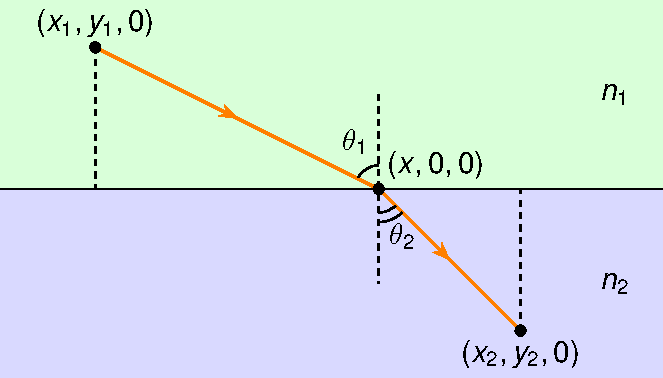
\includegraphics[width=0.7\textwidth]{Tuan9/Figures/Snellius_law.pdf}
    \caption{Tia sáng truyền qua hai môi trường có chiết suất khác nhau.}
    \label{fig:Snellius_law}
\end{figure}

\begin{enumerate}[label=(\alph*)]
    \item Chứng minh rằng thời gian truyền của tia sáng từ điểm \(\left( x_1, y_1, 0 \right)\) đến \(\left( x_2, y_2, 0 \right)\) được tính theo công thức:
    \[t = \dfrac{n_1}{c} \sqrt{(x-x_1)^2 + y_1^2} + \dfrac{n_2}{c} \sqrt{(x-x_2)^2 + y_2^2},\]
    \item Tìm giá trị của \(x\) theo \(x_1\), \(x_2\), \(y_1\), \(y_2\), \(n_1\) và \(n_2\) sao cho thời gian truyền \(t\) là nhỏ nhất. 
    \item Chứng minh định luật Snellius, tức là tỷ số giữa sin của góc tới và sin của góc khúc xạ là một hằng số:
    \[\dfrac{\sin \theta_1}{\sin \theta_2} = \dfrac{n_2}{n_1},\]
    trong đó \(\theta_1\) là góc tới và \(\theta_2\) là góc khúc xạ.
\end{enumerate}

